%%%%%%%%%%%%%%%%%%%%%%%%%%%%%%%%%%%%%%%%%
% Programming/Coding Assignment
% LaTeX Template
%
% This template has been downloaded from:
% http://www.latextemplates.com
%
% Original author:
% Ted Pavlic (http://www.tedpavlic.com)
%
% Note:
% The \lipsum[#] commands throughout this template generate dummy text
% to fill the template out. These commands should all be removed when 
% writing assignment content.
%
% This template uses a Perl script as an example snippet of code, most other
% languages are also usable. Configure them in the "CODE INCLUSION 
% CONFIGURATION" section.
%
%%%%%%%%%%%%%%%%%%%%%%%%%%%%%%%%%%%%%%%%%

%----------------------------------------------------------------------------------------
%	PACKAGES AND OTHER DOCUMENT CONFIGURATIONS
%----------------------------------------------------------------------------------------

\documentclass{article}

\usepackage{fancyhdr} % Required for custom headers
\usepackage{lastpage} % Required to determine the last page for the footer
\usepackage{extramarks} % Required for headers and footers
\usepackage[usenames,dvipsnames]{color} % Required for custom colors
\usepackage{graphicx} % Required to insert images
\usepackage{listings} % Required for insertion of code
\usepackage{courier} % Required for the courier font
\usepackage{lipsum} % Used for inserting dummy 'Lorem ipsum' text into the template

% Margins
\topmargin=-0.45in
\evensidemargin=0in
\oddsidemargin=0in
\textwidth=6.5in
\textheight=9.0in
\headsep=0.25in

\linespread{1.1} % Line spacing

% Set up the header and footer
\pagestyle{fancy}
\lhead{\hmwkAuthorName} % Top left header
\chead{\hmwkClass\ (\hmwkClassInstructor\ \hmwkClassTime): \hmwkTitle} % Top center head
\rhead{\firstxmark} % Top right header
\lfoot{\lastxmark} % Bottom left footer
\cfoot{} % Bottom center footer
\rfoot{Page\ \thepage\ of\ \protect\pageref{LastPage}} % Bottom right footer
\renewcommand\headrulewidth{0.4pt} % Size of the header rule
\renewcommand\footrulewidth{0.4pt} % Size of the footer rule

\setlength\parindent{0pt} % Removes all indentation from paragraphs

%----------------------------------------------------------------------------------------
%	CODE INCLUSION CONFIGURATION
%----------------------------------------------------------------------------------------

\definecolor{MyDarkGreen}{rgb}{0.0,0.4,0.0} % This is the color used for comments
\lstloadlanguages{Perl} % Load Perl syntax for listings, for a list of other languages supported see: ftp://ftp.tex.ac.uk/tex-archive/macros/latex/contrib/listings/listings.pdf
\lstset{language=Perl, % Use Perl in this example
        frame=single, % Single frame around code
        basicstyle=\small\ttfamily, % Use small true type font
        keywordstyle=[1]\color{Blue}\bf, % Perl functions bold and blue
        keywordstyle=[2]\color{Purple}, % Perl function arguments purple
        keywordstyle=[3]\color{Blue}\underbar, % Custom functions underlined and blue
        identifierstyle=, % Nothing special about identifiers                                         
        commentstyle=\usefont{T1}{pcr}{m}{sl}\color{MyDarkGreen}\small, % Comments small dark green courier font
        stringstyle=\color{Purple}, % Strings are purple
        showstringspaces=false, % Don't put marks in string spaces
        tabsize=5, % 5 spaces per tab
        %
        % Put standard Perl functions not included in the default language here
        morekeywords={rand},
        %
        % Put Perl function parameters here
        morekeywords=[2]{on, off, interp},
        %
        % Put user defined functions here
        morekeywords=[3]{test},
       	%
        morecomment=[l][\color{Blue}]{...}, % Line continuation (...) like blue comment
        numbers=left, % Line numbers on left
        firstnumber=1, % Line numbers start with line 1
        numberstyle=\tiny\color{Blue}, % Line numbers are blue and small
        stepnumber=5 % Line numbers go in steps of 5
}

% Creates a new command to include a perl script, the first parameter is the filename of the script (without .pl), the second parameter is the caption
\newcommand{\pythonscript}[2]{
\begin{itemize}
%\item[]\lstinputlisting[caption=#2,label=#1]{#1.py}
\end{itemize}
}

%----------------------------------------------------------------------------------------
%	DOCUMENT STRUCTURE COMMANDS
%	Skip this unless you know what you're doing
%----------------------------------------------------------------------------------------

% Header and footer for when a page split occurs within a problem environment
\newcommand{\enterProblemHeader}[1]{
\nobreak\extramarks{#1}{#1 continued on next page\ldots}\nobreak
\nobreak\extramarks{#1 (continued)}{#1 continued on next page\ldots}\nobreak
}

% Header and footer for when a page split occurs between problem environments
\newcommand{\exitProblemHeader}[1]{
\nobreak\extramarks{#1 (continued)}{#1 continued on next page\ldots}\nobreak
\nobreak\extramarks{#1}{}\nobreak
}

\setcounter{secnumdepth}{0} % Removes default section numbers
\newcounter{homeworkProblemCounter} % Creates a counter to keep track of the number of problems

\newcommand{\homeworkProblemName}{}
\newenvironment{homeworkProblem}[1][Problem \arabic{homeworkProblemCounter}]{ % Makes a new environment called homeworkProblem which takes 1 argument (custom name) but the default is "Problem #"
\stepcounter{homeworkProblemCounter} % Increase counter for number of problems
\renewcommand{\homeworkProblemName}{#1} % Assign \homeworkProblemName the name of the problem
\section{\homeworkProblemName} % Make a section in the document with the custom problem count
\enterProblemHeader{\homeworkProblemName} % Header and footer within the environment
}{
\exitProblemHeader{\homeworkProblemName} % Header and footer after the environment
}

\newcommand{\problemAnswer}[1]{ % Defines the problem answer command with the content as the only argument
\noindent\framebox[\columnwidth][c]{\begin{minipage}{0.98\columnwidth}#1\end{minipage}} % Makes the box around the problem answer and puts the content inside
}

\newcommand{\homeworkSectionName}{}
\newenvironment{homeworkSection}[1]{ % New environment for sections within homework problems, takes 1 argument - the name of the section
\renewcommand{\homeworkSectionName}{#1} % Assign \homeworkSectionName to the name of the section from the environment argument
\subsection{\homeworkSectionName} % Make a subsection with the custom name of the subsection
\enterProblemHeader{\homeworkProblemName\ [\homeworkSectionName]} % Header and footer within the environment
}{
\enterProblemHeader{\homeworkProblemName} % Header and footer after the environment
}

%----------------------------------------------------------------------------------------
%	NAME AND CLASS SECTION
%----------------------------------------------------------------------------------------

\newcommand{\hmwkTitle}{Assignment\ \#3} % Assignment title
\newcommand{\hmwkDueDate}{Thursday,\ October\ 2,\ 2014} % Due date
\newcommand{\hmwkClass}{CS\ 595} % Course/class
\newcommand{\hmwkClassTime}{4:20PM} % Class/lecture time
\newcommand{\hmwkClassInstructor}{Dr Nelson} % Teacher/lecturer
\newcommand{\hmwkAuthorName}{VICTOR NWALA} % Your name

%----------------------------------------------------------------------------------------
%	TITLE PAGE
%----------------------------------------------------------------------------------------

\title{
\vspace{2in}
\textmd{\textbf{\hmwkClass:\ \hmwkTitle}}\\
\normalsize\vspace{0.1in}\small{Due\ on\ \hmwkDueDate}\\
\vspace{0.1in}\large{\textit{\hmwkClassInstructor\ \hmwkClassTime}}
\vspace{3in}
}

\author{\textbf{\hmwkAuthorName}}
\date{} % Insert date here if you want it to appear below your name

%----------------------------------------------------------------------------------------

\begin{document}

\maketitle

%----------------------------------------------------------------------------------------
%	TABLE OF CONTENTS
%----------------------------------------------------------------------------------------

%\setcounter{tocdepth}{1} % Uncomment this line if you don't want subsections listed in the ToC

\newpage
\tableofcontents
\newpage

%----------------------------------------------------------------------------------------
%	PROBLEM 1
%----------------------------------------------------------------------------------------

% To have just one problem per page, simply put a \clearpage after each problem

\begin{homeworkProblem}
1.  Download the 1000 URIs from assignment \#2.  ``curl", ``wget", or
``lynx" are all good candidate programs to use.  We want just the
raw HTML, not the images, stylesheets, etc.

%Listing\ref{downloadPage.py} shows a Python script.
\lstinputlisting[breaklines=true, caption=Python script to download html pages]{downloadPage.py}
This script downloads html pages, saves them in text files and places them in a folder called Html. The files are also saved with their respective md5 encrypted names.
\begin{figure}
      \centering
      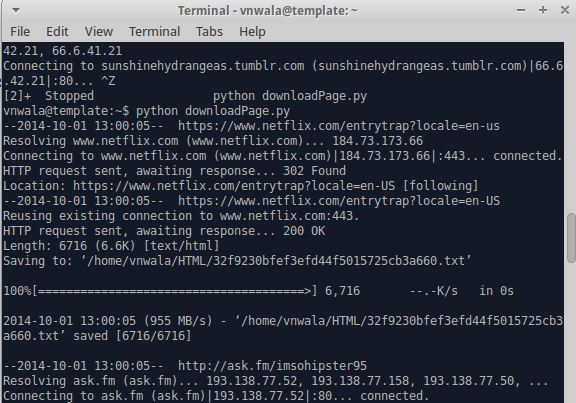
\includegraphics[width=4.0 in]{downloadPage} 
      \caption{downloadPage.py at work}
      \label{downloadPage.py at work}
\end{figure}
%Listing\ref{downloadText.py} shows a Python script.
\lstinputlisting[breaklines=true, caption=Python script to get text from html pages]{downloadText.py}
This script downloads the text content of all the urls and stores the with the md5 names into a file.
\begin{figure}
      \centering
      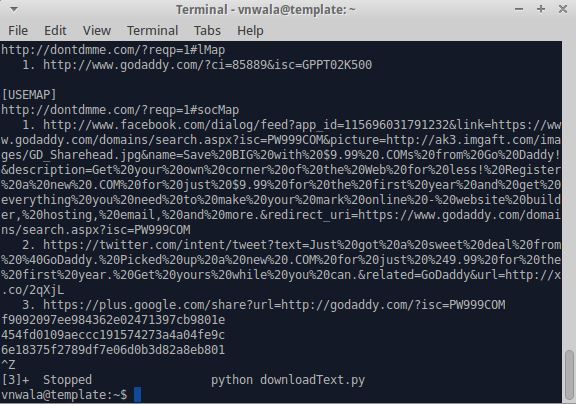
\includegraphics[width=4.0 in]{downloadText} 
      \caption{downloadText.py at work}
      \label{downloadText.py at work}
\end{figure}
\begin{figure}
      \centering
      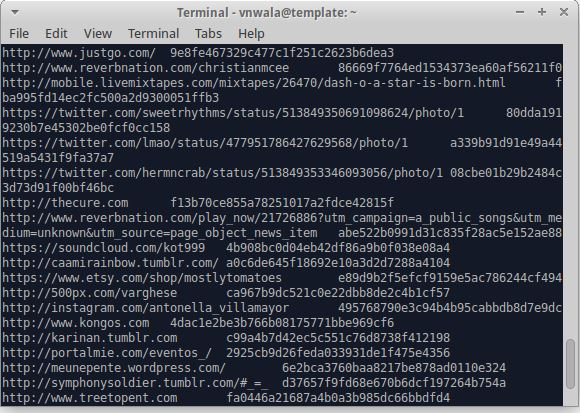
\includegraphics[width=4.0 in]{getHashes} 
      \caption{getHashes.py at work}
      \label{getHashes.py at work}
\end{figure}
%Listing\ref{getHashes.py} shows a Python script.
\lstinputlisting[breaklines=true, caption=Python script store URI and their md5 names]{getHashes.py}
This script converts URIs to md5 encryption  and stores the mapping.
\end{homeworkProblem}


%----------------------------------------------------------------------------------------
%	PROBLEM 2
%----------------------------------------------------------------------------------------
\begin{homeworkProblem}
2.  Choose a query term (e.g., ``shadow") that is not a stop word
(see week 4 slides) and not HTML markup from step 1 (e.g., ``http")
that matches at least 10 documents (hint: use ``grep" on the processed
files).  If the term is present in more than 10 documents, choose
any 10 from your list.  (If you do not end up with a list of 10
URIs, you've done something wrong).

%Listing\ref{wordCount.py} shows a Python script.
\lstinputlisting[breaklines=true, caption=Python script to calculate TF (wordCount.py)]{wordCount.py}
This script get the total word count of my text file, queries the word ``football" in all the text files, it then calculates TF for each file by diving the frequecy of the word (football) by the total word count for each file and stores the result.
\begin{figure}
      \centering
      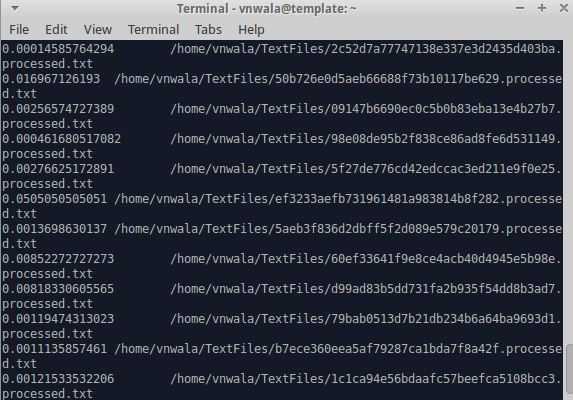
\includegraphics[width=4.0 in]{TF_cal} 
      \caption{wordCount.py at work}
      \label{wordCount.py at work}
\end{figure}

To calculte IDF, I used searched for the word ``football", I got 381,000,000 results. Still using the assumption that 20 billion pages are indexed by Bing:

IDF = logarithm to the base of 2 0f the result of (20,000,000,000/381,000,000) 


IDF = 5.71407

I chose 10 URI randomly and ranked them. The table displays ranking from the highest to the lowest.

\begin{table}[ht]
\caption{URL RANKING}% title of Table
\centering% used for centering table
\begin{tabular}{c c c c}
% centered columns (4 columns)
\hline\hline 
TF-IDF & TF & IDF & URI \\[0.5ex]% inserts table
%heading
\hline
0.078060999  & 0.0136612021858  & 5.71406519205585 & http://npcironmen.com \\
0.046759947  & 0.00818330605565 & 5.71406519205585 & http://www.maxpreps.com/national/national.htm \\ 
0.044381088  & 0.00776699029126 & 5.71406519205585 & http://qoly.jp\\ 
0.028244428  & 0.00494296577947 & 5.71406519205585 & http://www.chelseafc.com \\ 
0.006363106  & 0.0011135857461  & 5.71406519205585 & http://www.eonline.com\\ 
0.005771783  & 0.0010101010101  & 5.71406519205585 & http://twinsdaily.com/ \\ 
0.0029198084 & 0.00051098620337 & 5.71406519205585 & http://www.cracked.com \\ 
0.002835764  & 0.00049627791563 & 5.71406519205585 & http://www.latimes.com/entertainment/ \\ 
0.0026380726 & 0.00046168051708 & 5.71406519205585 & http://vkdiz.ru \\ 
0.0008334401 & 0.00014585764294 & 5.71406519205585 & http://www.lazywrita.com \\ [1ex]
\hline
\end{tabular}
\label{table:nonlin}
\end{table}

\end{homeworkProblem}

%----------------------------------------------------------------------------------------
%	PROBLEM 3
%----------------------------------------------------------------------------------------



\begin{homeworkProblem}
3.  Now rank the same 10 URIs from question \#2, but this time 
by their PageRank.  Use any of the free PR estimaters on the web,
such as:

http://www.prchecker.info/check\_page\_rank.php


http://www.seocentro.com/tools/search-engines/pagerank.html


http://www.checkpagerank.net/




To answer this question, I used http://www.prchecker.info/check\_page\_rank.php, to check the ranks of the respective URIs.
The table displays ranking from the highest to the lowest.
\begin{table}[ht]
\caption{URL RANKING USING http://www.prchecker.info/check\_page\_rank.php }% title of Table
\centering% used for centering table
\begin{tabular}{ c c c}
% centered columns (3 columns)
\hline\hline 
URI & PAGE RANK & NORMALIZED VALUES \\[0.5ex]% inserts table
%heading
\hline
http://www.maxpreps.com/national/national.htm & 8/10 & 1  \\ 
http://www.chelseafc.com/ & 7/10 & 0.875  \\ 
http://www.latimes.com/entertainment/ & 7/10 & 0.875  \\ 
http://www.eonline.com & 7/10 & 0.875  \\ 
http://www.cracked.com & 6/10 & 0.75  \\
http://qoly.jp & 5/10 & 0.675  \\ 
http://twinsdaily.com/ & 4/10 & 0.5  \\
http://vkdiz.ru & 2/10 & 0.25  \\ 
http://npcironmen.com & 0/10 & 0  \\ 
http://www.lazywrita.com & 0/10 & 0  \\ [1ex] 
\hline
\end{tabular}
\label{table:nonlin}
\end{table}


Comparing both ranking schemes in 2 and 3, of the URIs I noticed they were not the same but in some way consistent except few exceptions. Some links rank high on both methods, some intermediate on both and others low, even if their ranking positions differ. 
I observed that links which have not been indexed by google do not have a page rank using the PageRank scheme. Also the ranking system of this scheme is based on counting the number and quality of links to a page, hence giving them a rank in their order of importance.
\clearpage
\begin{figure}
      \centering
      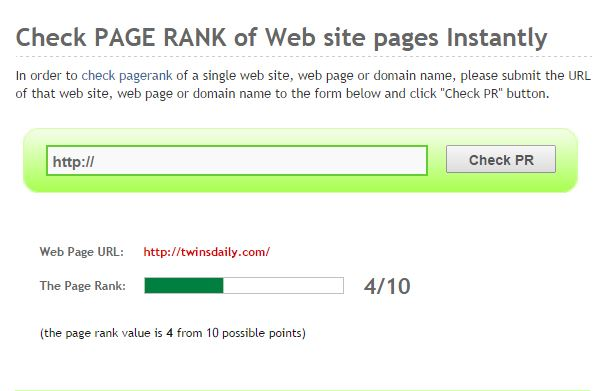
\includegraphics[width=4.0 in]{pageRank} 
      \caption{PAGE RANK SCREEN SHOT}
      \label{PAGE RANK SCREEN SHOT}
\end{figure}

\end{homeworkProblem}
%----------------------------------------------------------------------------------------

\end{document}
